% ##################################################################################################################
\section{The Philippines: Agent-Based Transport Simulation Model for Disaster Response Vehicles}
\label{sec:philippines}
\hfill \textbf{Author:} Elvira B. Yaneza

% ##################################################################################################################
The primary purpose of this study is to adopt an agent-based traffic simulation model to assist planning agencies in determining road traffic routes for exclusive use of \gls{drv} in the event of disaster. After the initial period of disaster, road network management is crucial to cope with the increase of travel demand for disaster response operations. Depending on the level of road damages, possible road closures may occur in the road network. The degraded road traffic routes of \gls{drv} will result in increase of travel time period from its source to destination.

The model is developed using agent-based simulation modeling paradigm implemented through the use of \gls{matsim}. Road traffic routes are generated using Dijkstra’s shortest path algorithm. \gls{matsim} output files store the routes by each agent. These routes represent the traffic routes for \gls{drv}, in which the travel time calculated in each route is equivalent to the running time of each agent in actual motion while traversing the shortest paths from source to destination. 

% ##################################################################################################################
\section{Literature Review}
Studies involving road traffic routing has generally use different modeling approaches and shortest path algorithms. Among studies using modeling approach, \citet[][]{LefebvreBalmer_TechRep_IVT_2007} used \gls{matsim} for \gls{largescale} agent-based transport simulation and investigated the variations of Dijkstra’s algorithm and A*-algorithm as well. Sumalee and Kurauchi [2] used Monte-Carlo simulation approach to approximate the capacity reliability of the network. The study was then used to evaluate the performances of traffic regulation policies with road network of Kobe city in Japan. Teknomo [3] multi-agent simulation modeling approach considered route probability as direct output of the simulation rather than an input to the network. Sanders and Schultes [4] outlined algorithms for route planning in transportation networks that run faster than Dijkstra’s algorithm. Their study focused on successful speedup techniques in static road network with fixed edge cost. Elalouf [5] model incorporated joint analysis of expected route time and its variance and used dynamic-programming shortest path algorithm as basis for a fully polynomial time approximation scheme. 

% ##################################################################################################################
\section{Design Details And Specifications}
% ..........................................
\paragraph{Element 1: Study Area}
During the occurrence of Tropical Storm Washi (Sendong), the most affected areas were those near the strip of Cagayan de Oro river [6]. Landslides near the river banks, flash floods, overflowing rivers and tributaries, caused some barangays having swept away during the occurrence of Tropical Depression Shanshan (Crising) [7]. The five major bridges mostly affected lie along Cagayan de Oro River connecting its two main lands, District 1 to the west and District 2 to the east, located in the province of Misamis Oriental, Philippines (see Figure~\ref{fig:philippines_fig1}). The designated road network coverage has a total area of approximately 73.2\.square kilometers which includes the riverside (see Figure~\ref{fig:philippines_fig3}). 

% ..........................................
\paragraph{Element 2: Road Network and Facilities}
The model involves three main entities: road network, facilities and population. Road network is described by two variables: nodes and links. It is represented using graphical representation and has 3\,847\,nodes and 9\,630\,directed links (see Figure~\ref{fig:philippines_fig2}). A stretch of a particular street may consist of nodes and links representing intersections and street sections, respectively. \gls{matsim} handles only one-way links. In this model, one-way attribute has a default value of 1 and modes attribute assigned only as car. Facilities are represented by its geographical coordinate locations in the network. It involves twenty one entities from the following agencies: 10\,hospitals with ambulance services, 3\,fire stations, 8\,police stations and 2\,evacuation centers. Facilities are mapped on its nearest links located in the road network.

% ..........................................
\paragraph{Element 3: Population and Demand Generation}
The population is composed of different types of \gls{drv} representing the major agents in the traffic simulation model. These are ambulances, fire trucks and police cars.  The hospitals, fire stations and police stations are assigned as origins of agents, where vehicles start and end their activities, whereas evacuation centers are assigned as destinations of agents. Population is characterized by four variables: person, plan, act and leg. The leg variable is characterized by mode that defines the type of vehicle, assigned as car. The model advances by performing traffic routing activities. Each traffic routing activity, seven events are processed in the following sequence: end activity event, agent departure event, wait to link event, enter link event, leave link event, agent arrival event and start activity event. The end activity event initiates the agent to depart from the facility of origin and back again in the same flow of events. 

% ##################################################################################################################
\section{Model Scenarios} \ah{do we need to use a different term than scenario here? However, these are \emph{actually} scenarios.}
The simulation model was applied to the network of Cagayan de Oro City in Philippines. Two scenarios were assumed.

% ..........................................
\paragraph{Scenario 1: No Bridge Closures}
The scenario was based on disaster response operations right after the occurrence of disaster. The operations took place in Cagayan de Oro City. The scenario has two evacuation centers identified, (1) Balulang Elementary School Evacuation Area located at the west side of Cagayan de Oro and (2) Burgos Barangay Hall Area located at the east side of the city. The road network has 21\,facilities as origins of agents having 3 to 4\,\gls{drv} in each, traversing the network into 2\,different evacuation centers. A total of 67\,\gls{drv} joined the operations over the time and 50\,additional vehicles coming from private institutions traveling on their own rescue operations with different origins and destinations. No road obstructions were considered so traffic movements can access all five bridges defined in the network (see Figure~\ref{fig:philippines_fig4}). During the simulation run, \gls{drv} were expected to pass the nearest bridge on its trip to the destinations or evacuation areas. Thus, passing only the routes that gave shortest time traveled.

% ..........................................
\paragraph{Scenario 2: With Bridge Closures}
In this scenario, road obstructions were represented as bridge closures in the network. The link ids of the identified bridges for closure were required as the data needed to run the java class for road closure generation. In the experiment performed, the link ids of the following three bridges were entered; Carmen Bridge, Rotunda Bridge and Marcos Bridge. The same two evacuation areas and fifty additional vehicles were considered in the experiment. This time considering road obstructions of three bridges only. The \gls{drv} and other vehicles were expected to pass only to the two remaining bridges not included in the road closure generation; Taguanao Bridge and Kauswagan-Puntod Bridge. The expectation of vehicle movements was met as seen during the visualization of the output (see Figure~\ref{fig:philippines_fig5}). 

% ##################################################################################################################
\section{Validation} 
% ..........................................
\paragraph{Face Validation from Field Experts}
The goal was to verify and validate if the simulation model had a reasonable representation of the real-world system and its conformance in the design and operational behavior specifications. Four domain experts were invited from the field of traffic engineering, computing, planning and management for the face validation. Two evaluators were invited from the academe, one was a Transportation Engineering and Built Environment Specialist and the other was a Computing Scientist. The other two evaluators were from the local government units, one was handling management and administration as Technical Supervisor from Road and Traffic Administration Office and the second was involved in planning as Coordinator of Cagayan de Oro City Planning Office. Either accepting or rejecting, the field experts evaluated the simulation model in terms of reasonableness based on their field of expertise. Generally, the four evaluators verified and accepted the design specifications of the simulation model as well as validated and accepted the operational behavior of the simulation model.

% ..........................................
\paragraph{Travel Time Validation Using Test Car Technique and Simulation Model Results}
Looking at the plans file, from both scenarios, it was found out that the calculated travel time resulted from the simulation was actually equal to the amount of running time that the vehicle was in actual motion. The running time was computed as equal to the difference between the travel time and stopped time delay. Actual measurement of travel time and delay using test car technique [8] and travel time using the simulation model were compared. Delay time was the time lost by traffic due to traffic friction, traffic control devices and geometric designs. The actual running time computed was only 36\,\% from the actual total travel time measured due to the amount of travel time delay. The difference between the actual running time computed and running time resulted from the simulation model was mainly caused by the vehicle speed ranges. 

% ##################################################################################################################
\section{Achieved Results}
% ..........................................
\paragraph{Scenario 1: No Bridge Closures}
Based on the generated events file, there were 667\,directed links used by agents representing the \gls{drv}. It was about 6.9\,\% of the total 9\,630\,directed links in the network. The events file stored all activities of 117\,agents, 67\,agents represented the \gls{drv} and 50\,agents represented the additional other vehicles. Finally, when no bridge obstruction occurred, the \gls{drv} coming from 86\,\% of the entities passed by the Carmen Bridge. For faster road traffic access, it was suggested that Carmen Bridge shall be declared exclusive for \gls{drv} during disaster response together with the 667\,directed links.

% ..........................................
\paragraph{Scenario 2: With Bridge Closures}
Results showed that there were 841\,directed links used by agents representing the \gls{drv}, about 8.7\,\% of the total 9\,630\,directed links in the network. Note that three bridges (i.e.,\,Marcos Bridge, Carmen Bridge and Rotunda Bridge) were considered for road closures. \gls{drv} originated from 90\,\% of the entities passed by Kauswagan-Puntod Bridge. Therefore, it was suggested that this bridge and the 841\,directed links were potential candidates in declaring routes for exclusive use of \gls{drv}.

% ################################################################################################################## 
\section{Conclusions}
This study shows that the simulation model has a reasonable representation of the real-world system as verified and validated by the four field domain experts. The results of the study prove the exclusive traffic routing system through the shortest path routes generated by Dijkstra’s algorithm. The results can then be utilized by traffic management decision-makers in determining traffic routes for exclusive use of disaster response vehicles in disaster events.

% ##################################################################################################################
\paragraph{Acknowledgements}
The author wishes to acknowledge the guidance and information received from the developers of \gls{matsim}, Prof. Dr. Nagel Kai of Transport Systems Planning and Transport Telematics at the Institute for Land and Sea Transport Systems, in Berlin, Germany and Dr. Marcel Rieser of Senozon AG in Switzerland. The author would also like to thank Engr. Gerardo S. Doroja for several discussions we had in the implementation of this model.

% ##################################################################################################################
\createfigure%
{Cagayan de Oro City, Philippines urban road network}%
{Cagayan de Oro City, Philippines urban road network}%
{\label{fig:philippines_fig1}}%
{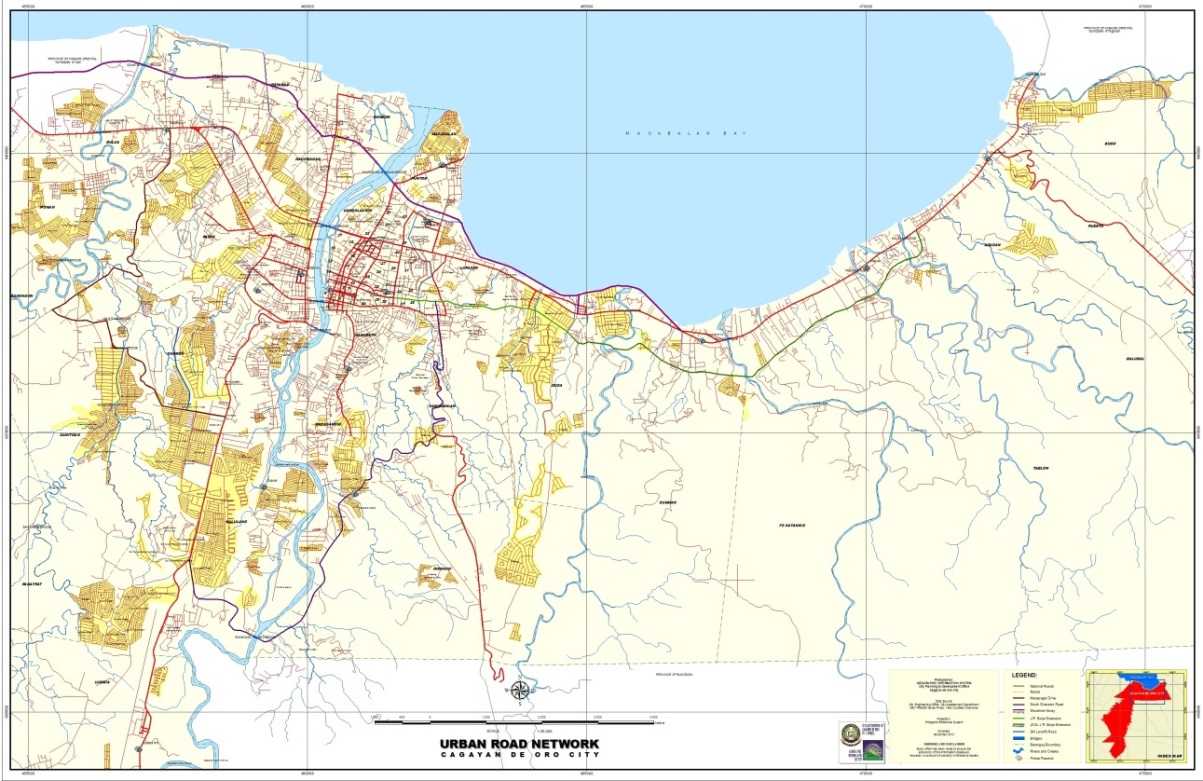
\includegraphics[width=0.85\textwidth, angle=0]{./using/figures/philippines_fig1.png}}%
{GIS City Planning Office, 2012}

\createfigure%
{Spatial coverage of the road network and locations of facilities in the network}%
{Spatial coverage of the road network and locations of facilities in the network: It has 73.2\,square kilometers which includes the land and surrounding river and coastal areas. The facilities are mapped based on its actual geographical x and y coordinates in the road network. There are 23\,facilities located in its nearest link in the network. These are 10\,hospitals, 3\,fire stations, 8\,police stations and 2\,evacuation centers.}%
{\label{fig:philippines_fig3}}%
{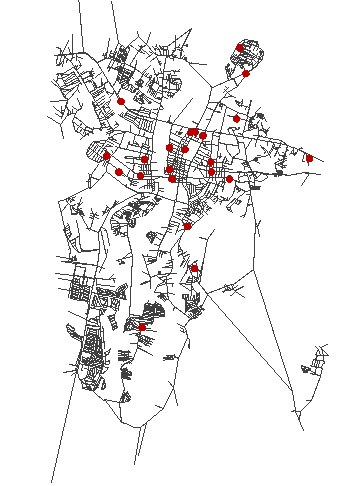
\includegraphics[width=0.85\textwidth, angle=0]{./using/figures/philippines_fig3.png}}%
{}

\createfigure%
{Nodes and links representation}%
{Nodes and links representation: Road Network has 3\,837\,nodes representing road intersections and 9\,630\,links representing the streets. It includes five major bridges along Cagayan River: A. Kauswagan-Puntod Bridge, B. Maharlika Bridge (formerly known as Marcos Bridge), C. Gov. Ysalina Bridge (formerly known as Carmen Bridge), D. Kagay-an Bridge (Rotunda Bridge) and E. Emmanuel Pelaez Bridge.}%
{\label{fig:philippines_fig2}}%
{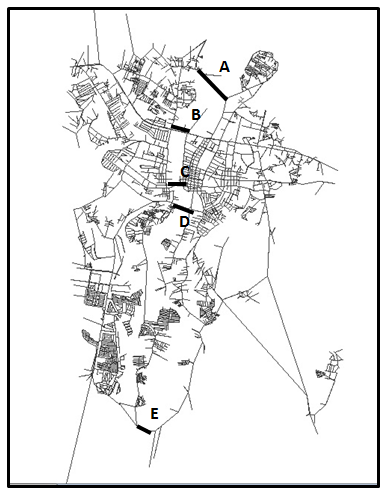
\includegraphics[width=0.85\textwidth, angle=0]{./using/figures/philippines_fig2.png}}%
{}

\createfigure%
{Screenshot of SCENARIO~1}%
{Screenshot of SCENARIO~1 (without bridge closures) using agent~ID\#4. \protect\gls{drv} trip starting from the Sabal Hospital (Origin) passing Carmen Bridge (Gov. Ysalina Bridge) going to Balulang Evacuation Center dropping point (destination) then back to its origin.}%
{\label{fig:philippines_fig4}}%
{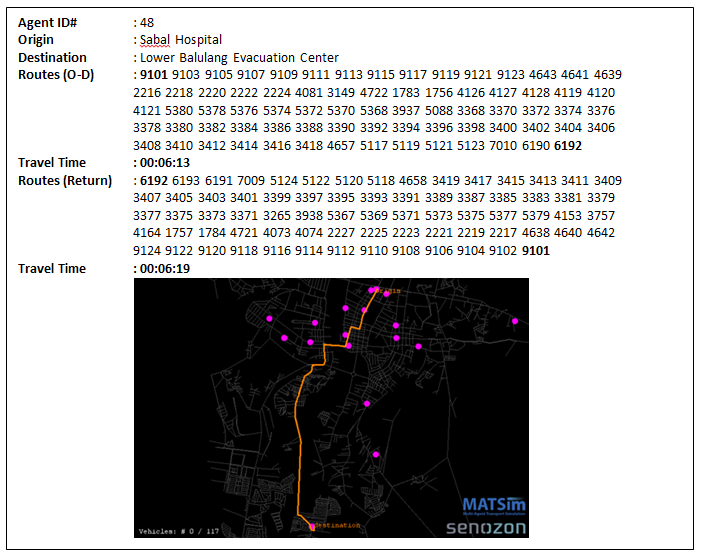
\includegraphics[width=0.85\textwidth, angle=0]{./using/figures/philippines_fig4.png}}%
{}

\createfigure%
{Screenshot of SCENARIO~2}%
{Screenshot of SCENARIO~2 (with bridge closures) using Agent~ID\#48. \protect\gls{drv} trip starting from the Sabal Hospital (Origin) passing Kauswagan-Puntod Bridge going to Balulang Evacuation Center dropping point (destination) then back to its origin.}%
{\label{fig:philippines_fig5}}%
{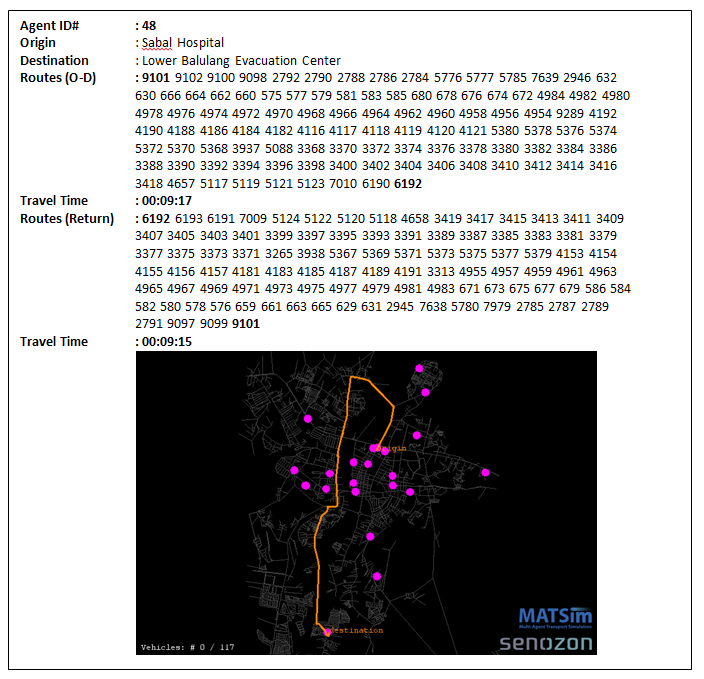
\includegraphics[width=0.85\textwidth, angle=0]{./using/figures/philippines_fig5.png}}%
{}

% ##################################################################################################################






 
